\chapter{Linear Combinations of Vectors}

In the introductory linear algebra chapter, you learned that vectors and 
matrices can be rotated, inverted, and added. In this chapter, we will explore 
linear combinations of vectors and the span of group of vectors. The 
\textbf{span}\index{span} of a group of vectors is the set of vectors that can 
be made with linear combinations of the original group of vectors. We will 
offer mathematical and visual explanations later in the chapter. First, let's 
examine linear combinations. 

A linear combination is simply the addition of vectors with leading scalar 
multipliers. For example, $3 \left[ 2, -1 \right] + 2 \left[ 3, 5 \right]$ is 
a linear combination of the vectors $\left[ 2, -1 \right]$ and $\left[ 3, 5 
\right]$. Another way to say this is:

\begin{mdframed}[style = important, frametitle = {Linear Combination of 
Vectors}]
A linear combination of a list of $n$ vectors, $\mathbf{v_1}, \mathbf{v_2}, \dots, \mathbf{v_n}$ takes the form:
$$a_1 \mathbf{v_1} + a_2 \mathbf{v_2} + \dots + a_n \mathbf{v_n}$$

where $a_1, a_2, \cdots, a_n \in \mathbb{R}$
\end{mdframed}

\textbf{Example}: Find a linear combination of $\left[ 2, 1, -3 \right]$ and 
$\left[ 1, -2, 4 \right]$ that gives the vector $\left[ 17, -4, 2 \right]$.

\textbf{Solution}: We are looking for $a_1$ and $a_2$ such that:
$$a_1 \left[ 2, 1, -3 \right] + a_2 \left[ 1, -2, 4 \right] = \left[17, -4, 2 
\right]$$

Looking at each dimension separately, we get the system of equations:
$$2 a_1 + 1 a_2 = 17$$
$$1 a_1 - 2 a_2 = -4$$
$$-3 a_1 + 4 a_2 = 2$$

If we can solve this system of equations, we will find $a_1$ and $a_2$. Let's 
multiply the first equation by 2 and add it to the second equation:
$$2 \left[ 2 a_1 + a_2 \right] + \left[ a_1 - 2 a_2 \right] = 2 \left( 17 
\right) + -4$$
$$4 a_1 + 2 a_2 + a_1 - 2 a_2 = 34 - 4$$
$$5 a_1 = 30$$
$$a_1 = 6$$

Now we can take $a_1$ and substitute it back into any equation in our system 
to find $a_2$. Let's use the third equation:
$$-3 \left( 6 \right) + 4 a_2 = 2$$
$$ -18 + 4 a_2 = 2$$
$$4 a_2 = 20$$
$$a_2 = 5$$

Since we used all 3 equations, we know $a_1 = 6$ and $a_2 = 5$ are solutions 
to all 3 equations. If we had only used the first two equations to find $a_1$ 
and $a_2$, we would want to substitute our values back into the third equation 
to make sure our solution holds for that equation also. 

Therefore, $6 \left[ 2, 1, -3 \right] + 5 \left[ 1, -2, 4 \right] = \left[ 17, 
-4, 2 \right]$.

\begin{Exercise}[title = {Linear Combinations}, label = combo]
Find a linear combination of the first two vectors that yields the third 
vector. 
\begin{enumerate}
\item $\left[1, 2 \right]$, $\left[ -3, 1 \right]$, $\left[ 4, 5 \right]$
\item $\left[ 9, 4 \right]$, $\left[ 0, 1 \right]$, $\left[ -5, 3 \right]$
\item $\left[ 7, -2 \right]$, $\left[ -8, 4 \right]$, $\left[ 6, -2 \right]$
\end{enumerate}
\vspace{50mm}
\end{Exercise}

\begin{Answer}[ref = combo]
\begin{enumerate}
    \item We are looking for $a_1$ and $a_2$ such that:
    $$a_1 \left[ 1, 2 \right] + a_2 \left[ -3, 1 \right] = \left[ 4, 5 
    \right]$$
    Which creates the system of equations:
    $$a_1 - 3 a_2 = 4$$
    $$2 a_1 + a_2 = 5$$

    We can multiply the first equation by $-2$ and add it to the second to 
    solve for $a_2$:
    $$-2 \left( a_1 - 3 a_2 \right) + 2 a_1 + a_2 = -2 \left( 4 \right) + 5$$
    $$6 a_2 + a_2 = -8 + 5$$
    $$7 a_2 = -3$$
    $$a_2 = -\frac{3}{7}$$

    Substituting $a_2$ back into an equation and solving for $a_1$:
    $$a_1 - 3 \left( -\frac{3}{7} \right) = 4$$
    $$a_1 + \frac{9}{7} = 4$$
    $$a_1 = \frac{19}{7}$$

    Therefore, $\frac{19}{7} \left[ 1, 2 \right] - \frac{3}{7} \left[ -3, 1 
    \right] = \left[ 4, 5 \right]$.

    \item We are looking for $a_1$ and $a_2$ such that:
    $$a_1 \left[ 9, 4 \right] + a_2 \left[ 0, 1 \right] = \left[ -5, 3 \right]$$
    Which creates the system of equations:
    $$9 a_1 = -5$$
    $$4 a_1 + a_2 = 3$$

    We can find $a_1$ from the first equation:
    $$a_1 = -\frac{5}{9}$$

    Substituting for $a_1$ back into the second equation and solving for $a_2$:
    $$4 \left( -\frac{5}{9} \right) + a_2 = 3$$
    $$a_2 - \frac{20}{9} = 3$$
    $$a_2 = \frac{47}{9}$$

    Therefore, $-\frac{5}{9} \left[ 9, 4 \right] + \frac{47}{9} \left[ 0, 1 
    \right] = \left[ -5, 3 \right]$.

    \item We are looking for $a_1$ and $a_2$ such that:
    $$a_1 \left[ 7, -2 \right] + a_2 \left[ -8, 4 \right] = \left[ 6, -2 
    \right]$$

    Which yields the system of equations:
    $$7 a_1 - 8 a_2 = 6$$
    $$-2 a_1 + 4 a_2 = -2$$

    Doubling the second equation and adding it to the first:
    $$7 a_1 - 8 a_2 + 2 \left( -2 a_1 + 4 a_2 \right) = 6 + 2 \left( -2 
    \right)$$
    $$7 a_1 - 8 a_2 - 4 a_1 + 8 a_2 = 6 - 4$$
    $$3 a_1 = 2$$
    $$a_1 = \frac{2}{3}$$

    Substituting for $a_1$ back into the second equation and solving for $a_2$:
    $$-2 \left( \frac{2}{3} \right) + 4 a_2 = -2$$
    $$-\frac{4}{3} + 4 a_2 = -2$$
    $$4 a_2 = -\frac{2}{3}$$
    $$a_2 = -\frac{1}{6}$$

    Therefore, $\frac{2}{3} \left[ 7, -2 \right] - \frac{1}{6} \left[ -8, 4 
    \right] = \left[ 6, -2 \right]$
\end{enumerate}
\end{Answer} 

Sometimes, a set of vectors cannot be combined to make a specific vector. Take 
the pair of vectors we have looked at before: $\left[ 2, 1, -3 \right]$ and 
$\left[ 1, -2, 4 \right]$. Can we find a combination to make vector $\left[ 
17, -4, 5 \right]$? Let's try. We define $a_1$ and $a_2$ such that:
$$a_1 \left[ 2, 1, -3 \right] + a_2 \left[ 1, -2, 4 \right] = \left[ 17, -4, 5 
\right]$$

Which creates the system of equations:
$$2 a_1 + a_2 = 17$$
$$a_1 - 2 a_2 = -4$$
$$-3 a_1 + 4 a_2 = 5$$

We have two variables ($a_1$ and $a_2$) and three equations. Let's use the 
first two to find $a_1$ and $a_2$, then check our answers by substituting our 
solutions into the third equation. First, we'll multiply the second equation 
by $-2$ and add that to the first equation:
$$2 a_1 + a_2 + \left( -2 \right) \left( a_1 - 2 a_2 \right) = 17 + \left( -2 
\right) \left( -4 \right)$$
$$2 a_1 + a_2 - 2 a_1 + 4 a_2 = 17 + 8$$
$$5 a_2 = 25$$
$$a_2 = 5$$

Substituting for $a_2$ back into the first equation and solving for $a_1$:
$$2 a_1 + 5 = 17$$
$$2 a_1 = 12$$
$$a_1 = 6$$

Now, let's check if $a_1 = 6$, $a_2 = 5$ is a solution to the third equation:
$$-3 \left( 6 \right) + 4 \left( 5 \right) = 5$$
$$-18 + 20 = 2 \neq 5$$

Therefore, there is no linear combination of the vectors $\left[ 2, 1, -3 
\right]$ and $\left[ 1, -2, 4 \right]$ that yields $\left[ 17, -4, 5 \right]$.

\section{Visualizing Linear Combinations}
First, let's look at what vectors can be made from linear combinations of the 
2-dimensional unit vectors $\textbf{i} = \left[ 1, 0 \right]$ and $\textbf{j} 
= \left[ 0, 1 \right]$. Suppose we are looking for a linear combination of 
\textbf{i} and \textbf{j} to create the vector $\left[ 3, -4 \right]$. We can 
find such a linear combination:
$$3\textbf{i} + \left( -4 \right) \textbf{j} = 3 \left[1, 0 \right] - 4 \left[ 
0, 1 \right] = \left[ 3, -4 \right]$$

In fact, with \textbf{i} and \textbf{j}, we can create any 2-dimensional 
vector. To prove this, consider a generic vector, $\textbf{z} = \left[ a, b 
\right]$, where $a, b \in \mathbb{R}$. We are looking for a linear combination 
of \textbf{i} and \textbf{j} such that:
$$c_1 \textbf{i} + c_2 \textbf{j} = \left[ a, b \right]$$

The above equation yields the system of equations:
$$c_1 \left( 1 \right) + c_2 \left( 0 \right) = a$$
$$c_1 \left( 0 \right) + c_2 \left( 1 \right) = b$$

And the solution to this system of equations is:
$$c_1 = a$$
$$c_2 = b$$

Therefore, using \textbf{i} and \textbf{j}, we can construct any vector in 
$\mathbb{R}^2$ (that is, any vector in the $xy$-plane). What about combinations 
of other vectors?

Let's consider linear combinations of two vectors: $\textbf{u} = \left[ 1, 2 
\right]$ and $\textbf{v} = \left[ -2, 1 \right]$. The vectors are shown in 
figure \ref{fig:u_and_v}. 

\begin{figure}[htbp]
    \centering
    \begin{tikzpicture}
        \begin{axis}[xmin = -3, xmax = 3, ymin = -3, ymax = 3, axis lines = 
        center, clip = false]
            \draw[blue, thick, -latex] (0, 0) -- (1, 2) node[above, black, 
            font = \scriptsize] {\textbf{u}};
            \draw[blue, thick, -latex] (0, 0) -- (2, 0) node[above, black, 
            font = \scriptsize] {\textbf{v}};
        \end{axis}
    \end{tikzpicture}
    \caption{The vectors $\textbf{u} = \left[ 1, 2 \right]$ and $\textbf{v} = 
    \left[ 2, 0 \right]$.}
    \label{fig:u_and_v}
\end{figure}

Suppose we want to construct the vector $\left[ -1, 4 \right]$. Since only 
\textbf{u} has value in the $y$-dimension, we can start by adding \textbf{u} 
vectors to reach $y = 4$ (see figure \ref{fig:just_u}). Next, we can use 
\textbf{v} vectors to reach $\left[ -1, 4 \right]$ (see figure \ref{fig:reach}). 

\begin{figure}[htbp]
    \centering
    \begin{tikzpicture}
        \begin{axis}[xmin = -3, xmax = 3, ymin = -3, ymax = 5, axis lines = 
        center, clip = false]
            \draw[blue, thick, -latex] (0, 0) -- (1, 2) node[above, black, 
            font = \scriptsize, xshift = -0.5cm, yshift = -0.5cm] {\textbf{u}};
            \draw[blue, thick, -latex] (1, 2) -- (2, 4) node[above, black, 
            font = \scriptsize, xshift = -0.5cm, yshift = -0.5cm] {\textbf{u}};
            \draw[red, fill = red] (-1, 4) circle (0.5mm);
            \draw[thin, black, latex-] (-1.1, 3.9) -- (-1.5, 3.5) node[below, 
            font = \scriptsize] {$\left[-1, 4 \right]$};
            \draw[red, dashed, -latex] (0,0) -- (-1, 4);
        \end{axis}
    \end{tikzpicture}
    \caption{To create vector $\left[ 4, -2 \right]$ with $\textbf{u} = \left[
    1, 2 \right]$ and $\textbf{v} = \left[2, 0 \right]$, we begin by adding two 
    \textbf{u} vectors to reach a $y$-value of 4.}
    \label{fig:just_u}
\end{figure}

\begin{figure}[htbp]
    \centering
    \begin{tikzpicture}
        \begin{axis}[xmin = -3, xmax = 3, ymin = -3, ymax = 5, axis lines = 
        center, clip = false]
            \draw[blue, thick, -latex] (0, 0) -- (1, 2) node[above, black, 
            font = \scriptsize, xshift = -0.5cm, yshift = -0.5cm] {\textbf{u}};
            \draw[blue, thick, -latex] (1, 2) -- (2, 4) node[above, black, 
            font = \scriptsize, xshift = -0.5cm, yshift = -0.5cm] {\textbf{u}};
            \draw[blue, thick, -latex] (2, 4) -- (0, 4) node[above, black, 
            font = \scriptsize, xshift = 1cm] {-\textbf{v}};
            \draw[blue, thick, -latex] (0, 4) -- (-1, 4) node[above, black, 
            font = \scriptsize, xshift = 0.5cm] {-0.5\textbf{v}};
            \draw[red, fill = red] (-1, 4) circle (0.5mm);
            \draw[thin, black, latex-] (-1.1, 3.9) -- (-1.5, 3.5) node[below, 
            font = \scriptsize] {$\left[-1, 4 \right]$};
            \draw[red, dashed, -latex] (0,0) -- (-1, 4);
        \end{axis}
    \end{tikzpicture}
    \caption{If $\textbf{u} = \left[1, 2 \right]$ and $\textbf{v} = \left[2, 0 
    \right]$, then $2\textbf{u} - 1.5 \textbf{v} = \left[-1, 4 \right]$.}
    \label{fig:reach}
\end{figure}

Using this method, we can imagine reaching any point in $\mathbb{R}^2$: we add 
or subtract as many \textbf{u} vectors as needed to reach the appropriate 
$y$-value, then add or subtract as many \textbf{v} vectors to reach the 
appropriate $x$-value.

Let's look at another pair of vectors: $\textbf{p} = \left[2, 2 \right]$ and 
$\textbf{q} = \left[ -1, -1 \right]$ (see figure \ref{fig:p_and_q}). Again, 
let's try to use \textbf{p} and \textbf{q} to construct the vector $\left[ -1, 
4 \right]$. We begin by using \textbf{p} to reach the $y$-value of 4 (see 
figure \ref{fig:just_p}).

\begin{figure}[htbp]
    \centering
    \begin{tikzpicture}
        \begin{axis}[xmin = -3, xmax = 3, ymin = -3, ymax = 5, axis lines = 
        center, clip = false]
            \draw[blue, thick, -latex] (0,0) -- (2, 2) node[above, black, 
            font = \scriptsize] {\textbf{p}};
            \draw[blue, thick, -latex] (0,0) -- (-1, -1) node[above, black, 
            font = \scriptsize] {\textbf{q}};
            \draw[black, fill = black] (0,0) circle (0.5mm);
        \end{axis}
    \end{tikzpicture}
    \caption{The vectors $\textbf{p} = \left[ 2, 2 \right]$ and $\textbf{q} = 
    \left[ -1, -1\right]$.}
    \label{fig:p_and_q}
\end{figure}

\begin{figure}[htbp]
    \centering
    \begin{tikzpicture}
        \begin{axis}[xmin = -3, xmax = 4, ymin = -3, ymax = 5, axis lines = 
        center, clip = false]
            \draw[blue, thick, -latex] (0,0) -- (2, 2) node[above, black, 
            font = \scriptsize, xshift = -0.6cm, yshift = -0.5cm] {\textbf{p}};
            \draw[blue, thick, -latex] (2, 2) -- (4, 4) node[above, black, 
            font = \scriptsize, xshift = -0.6cm, yshift = -0.5cm] {\textbf{p}};
            \draw[red, fill = red] (-1, 4) circle (0.5mm);
            \draw[black, fill = black] (0,0) circle (0.5mm);
            \draw[red, dashed, -latex] (0,0) -- (-1, 4);
            \draw[black, latex-] (-1.1, 3.9) -- (-1.6, 3.4) node[below, 
            font = \scriptsize] {$\left[ -1, 4 \right]$};
        \end{axis}
    \end{tikzpicture}
    \caption{Adding 2 \textbf{p} vectors gets us to the appropriate $y$-value 
    of 4.}
    \label{fig:just_p}
\end{figure}

But now we run into a problem: no matter how many \textbf{q} vectors we add or 
subtract, we just move along the \textbf{p} vector and never reach our goal of 
$\left[-1, 4 \right]$ (see figure \ref{fig:fail}). Notice that \textbf{p} and 
\textbf{q} lie on the same line (for a better visualization, refer back to 
\ref{fig:p_and_q}). When two vectors lie on the same line, we call them 
\textit{linearly dependent}\index{linearly dependent}. 

\begin{figure}[htbp]
    \centering
    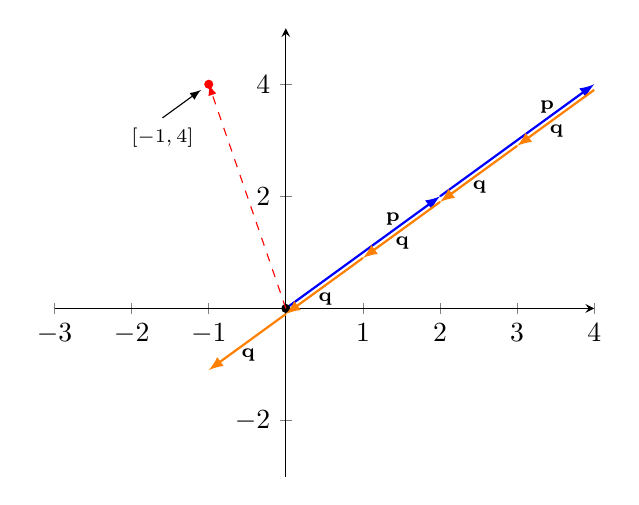
\begin{tikzpicture}
        \begin{axis}[xmin = -3, xmax = 4, ymin = -3, ymax = 5, axis lines = 
        center, clip = false]
            \draw[blue, thick, -latex] (0,0) -- (2, 2) node[above, black, 
            font = \scriptsize, xshift = -0.6cm, yshift = -0.5cm] {\textbf{p}};
            \draw[blue, thick, -latex] (2, 2) -- (4, 4) node[above, black, 
            font = \scriptsize, xshift = -0.6cm, yshift = -0.5cm] {\textbf{p}};
            \draw[red, fill = red] (-1, 4) circle (0.5mm);
            \draw[black, fill = black] (0,0) circle (0.5mm);
            \draw[red, dashed, -latex] (0,0) -- (-1, 4);
            \draw[black, latex-] (-1.1, 3.9) -- (-1.6, 3.4) node[below, 
            font = \scriptsize] {$\left[ -1, 4 \right]$};
            \draw[thick, orange, -latex] (4, 3.9) -- (3, 2.9) node[below, 
            black, font = \scriptsize, xshift = 0.5cm, yshift = 0.4cm] {
            \textbf{q}};
            \draw[thick, orange, -latex] (3, 2.9) -- (2, 1.9) node[below, 
            black, font = \scriptsize, xshift = 0.5cm, yshift = 0.4cm] {
            \textbf{q}};
            \draw[thick, orange, -latex] (2, 1.9) -- (1, 0.9) node[below, 
            black, font = \scriptsize, xshift = 0.5cm, yshift = 0.4cm] {
            \textbf{q}};
            \draw[thick, orange, -latex] (1, 0.9) -- (0, -0.1) node[below, 
            black, font = \scriptsize, xshift = 0.5cm, yshift = 0.4cm] {
            \textbf{q}};
            \draw[thick, orange, -latex] (0, -0.1) -- (-1, -1.1) node[below, 
            black, font = \scriptsize, xshift = 0.5cm, yshift = 0.4cm] {
            \textbf{q}};
        \end{axis}
    \end{tikzpicture}
    \caption{There is no linear combination of $\textbf{p} = \left[2, 2 
    \right]$ and $\textbf{q} = \left[ -1, -1 \right]$ that yields the vector 
    $\left[ -1, 4 \right]$.}
    \label{fig:fail}
\end{figure}

\section{Linearly Dependent Vectors}

Two vectors are linearly dependent if one is a multiple of the other. 
Mathematically, 

\begin{mdframed}[style = important, frametitle = {Linearly dependent vectors}]
Vectors $\textbf{u} = \left[ u_1, u_2, \dots, u_n \right]$ and $\textbf{v} = 
\left[ v_1, v_2, \dots, v_n \right]$ are linearly dependent if

$$\textbf{v} = a \textbf{u}$$

Where $a \in \mathbb{R}$ is a constant.
\end{mdframed}

If two vectors are linearly dependent, then linear combinations of those 
vectors can only create vectors that lie on the same line as the vectors. If 
two vectors are \textit{not} linearly dependent, then linear combinations of 
those vectors can create any vector in $\mathbb{R}^2$ (for two dimensions, we 
will discuss higher dimensions in the next chapter). 

\textbf{Example}: Which of the following 3 vectors are linearly dependent, if 
any? 
$\textbf{u} = \left[1, 2, 3 \right]$, $\textbf{v} = \left[ -3, 4, -1 \right]$, 
$\textbf{w} = \left[ 6, -8, 2 \right]$.

\textbf{Solution}: Two vectors are linearly dependent if one is a scalar 
multiple of the other. Let's compare \textbf{u} and \textbf{v}. Since the 
first component of \textbf{u} is 1 and the first component of \textbf{v} is 
-3, let's multiply \textbf{u} by -3 to see if we get \textbf{v}:
$$-3 \textbf{u} = -3 \left[ 1, 2, 3, \right] = \left[ -3, -6, -9 \right] \neq 
\textbf{v}$$

Therefore, \textbf{u} and \textbf{v} are \textit{not} linearly dependent. Now 
let's examine \textbf{v} and \textbf{w}. Again, we will use the first 
components: the first component of \textbf{w} is 6, so let's see if multiplying 
\textbf{v} by -2 yields \textbf{w}:
$$-2\textbf{v} = -2 \left[ -3, 4, -1 \right] = \left[ 6, -8, 2 \right] = 
\textbf{w}$$

Therefore, \textbf{v} and \textbf{w} are linearly dependent. Since we already 
know that \textbf{u} and \textbf{v} are not linearly dependent, we also know 
that \textbf{u} and \textbf{w} are also not linearly dependent. 

\begin{Exercise}[title = Linear Dependence, label = colinear]
Identify which, if any, of the following vectors are linearly dependent:
\begin{enumerate}
\item $\textbf{a} = \left[ -4, 1, 4 \right]$
\item $\textbf{b} = \left[ -4, 5, -3 \right]$
\item $\textbf{c} = \left[ 2, -4, 6 \right]$
\item $\textbf{d} = \left[ 1, -\frac{1}{4}, -1 \right]$
\item $\textbf{e} = \left[1, -2, 3 \right]$
\item $\textbf{f} = \left[ -6, \frac{3}{2}, 6 \right]$
\end{enumerate}
\end{Exercise}

\begin{Answer}[ref = colinear]
We see that $\frac{\textbf{a}}{-4} = -\frac{1}{4} \left[ -4, 1, 4 \right] = 
\left[ 1, -\frac{1}{4}, -1 \right] = \textbf{d}$. Additionally, $\frac{3}{2} 
\textbf{a} = \frac{3}{2} \left[ -4, 1, 4 \right] = \left[ -6, \frac{3}{2}, 6 
\right] = \textbf{f}$. Therefore, vectors \textbf{a}, \textbf{d}, and \textbf{f} 
are linearly dependent. 

We also see that $\frac{1}{2} \textbf{c} = \frac{1}{2} \left[ 2, -4, 6 \right] 
= \left[ 1, -2, 3 \right] = \textbf{e}$. Therefore, vectors \textbf{c} and 
\textbf{e} are linearly dependent. Vector \textbf{b} is not linearly dependent 
to any of the other vectors. 
\end{Answer}